%% Begin copyright
%%
%%  /home/jrf/Documents/books/Books20/Docs/Hjs/hjs_catalogue.tex
%%
%%   Part of the Books20 Project
%%
%%   Copyright 2022 James R. Fowler
%%
%%   All rights reserved. No part of this publication may be
%%   reproduced, stored in a retrival system, or transmitted
%%   in any form or by any means, electronic, mechanical,
%%   photocopying, recording, or otherwise, without prior written
%%   permission of the author.
%%
%%
%% End copyright
\documentclass[letterpaper]{book}

\usepackage{graphicx}
\usepackage{books20}
\usepackage[
  backend=biber,
  style=alphabetic,
]{biblatex}
\addglobalbib{../MasterBib.bib}
\addbibresource{hjs_baas_obit.bib}

%
% History
% created 11 June 2022
%
%----------------------------------------------------------
\begin{document}

\frontmatter
\pagestyle{empty}
\title{Catalogue of the Harlan J.~Smith Collection \\
  of Books in the Otto Struve Library \\
  of the McDonald Observatory, \\
  Fort Davis, Texas}
\author{compiled by James R. Fowler}
\date{copy of \today}
\maketitle
\clearpage

\vspace*{5 in}
\centerline{Copyright \copyright 2022 McDonald Observatory}
\centerline{Fort Davis, Texas}
\clearpage

\pagestyle{plain}
\begin{figure}
  \centering
  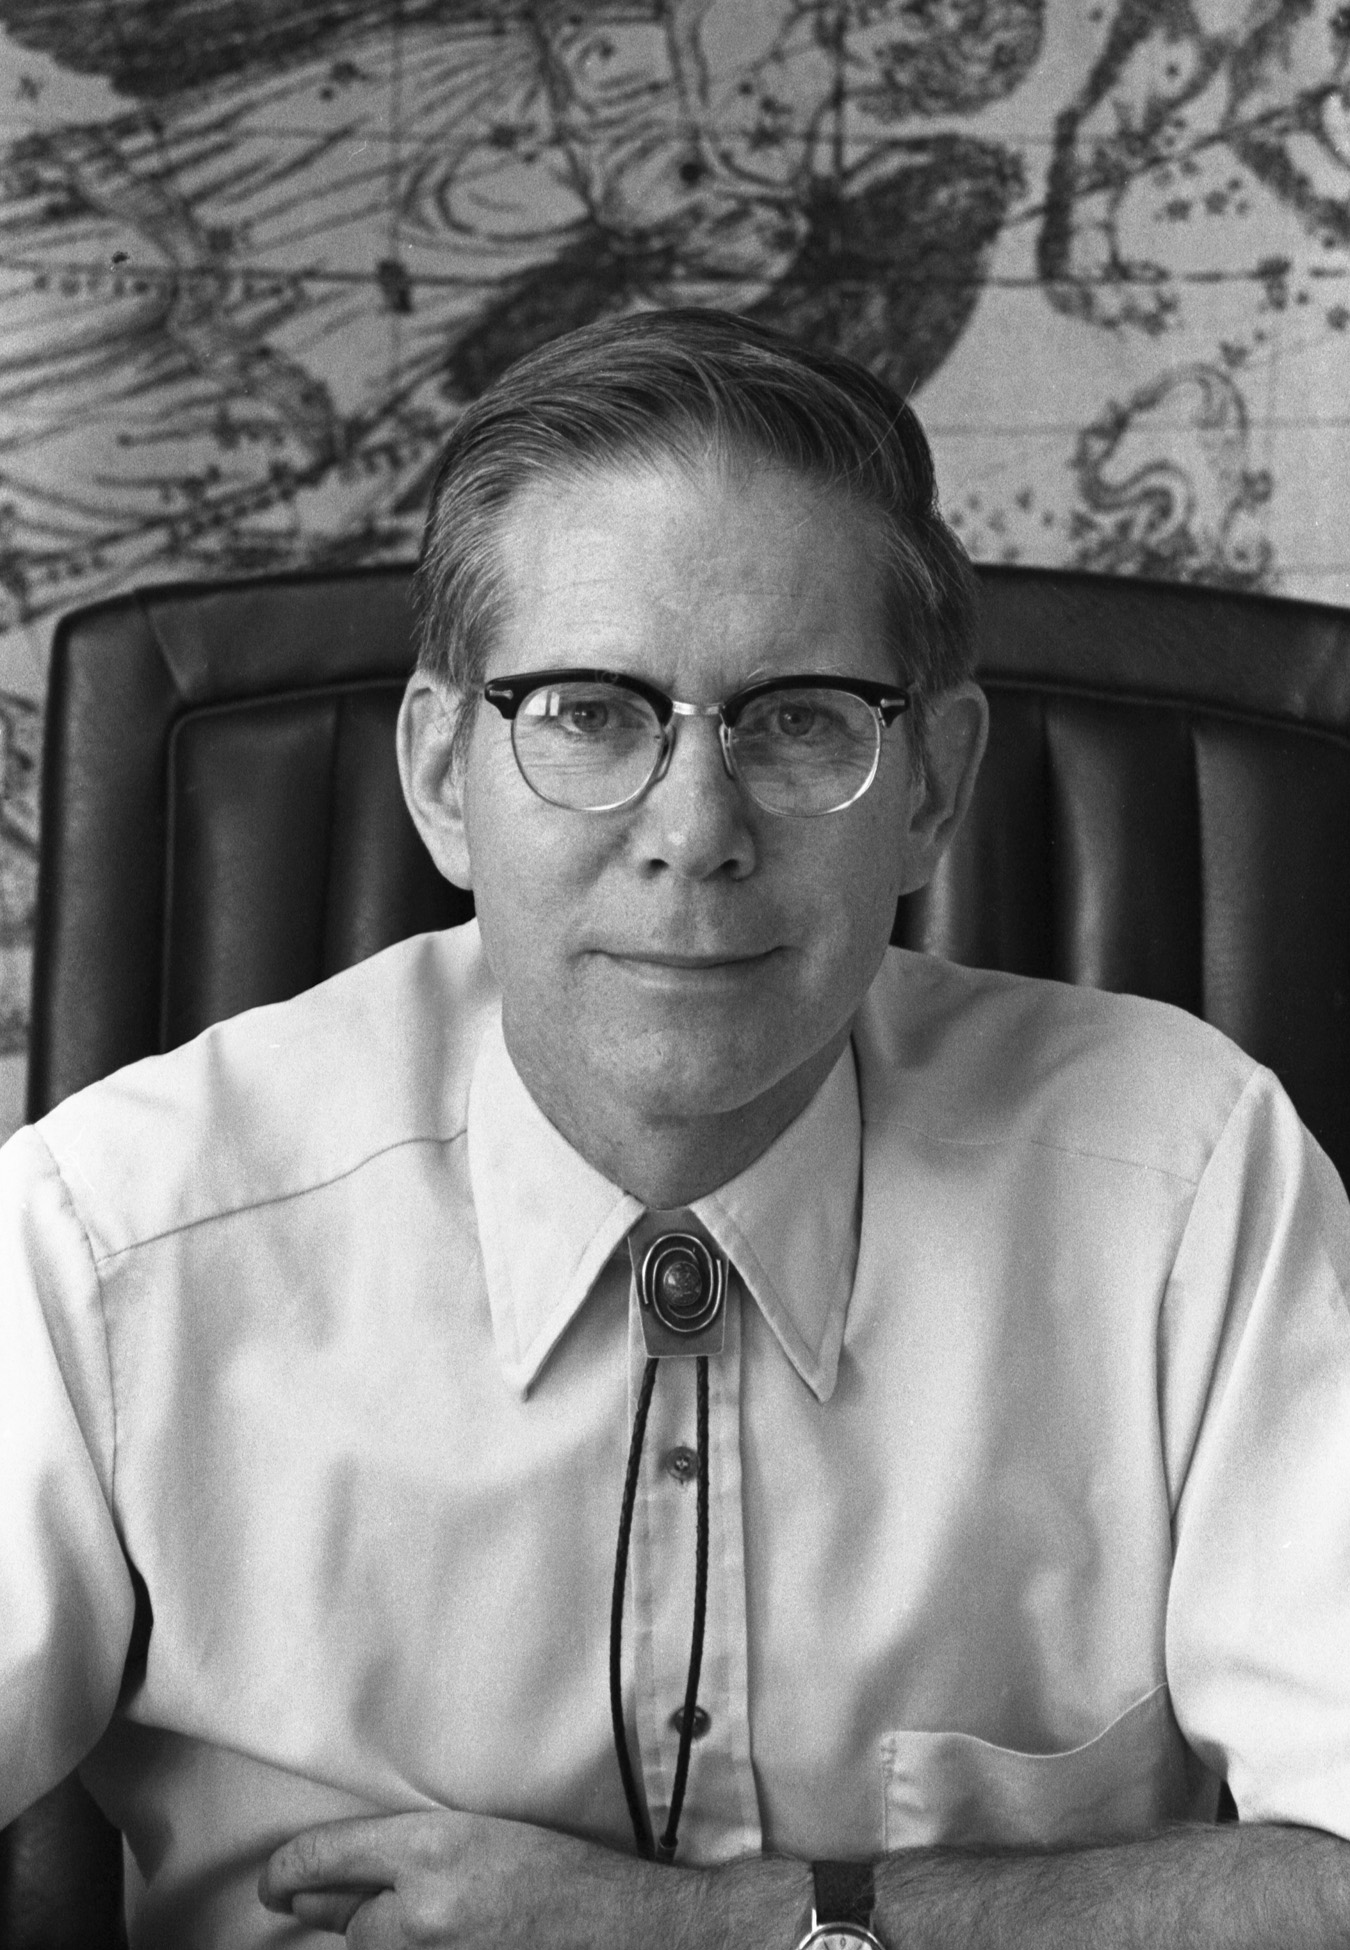
\includegraphics{hjs_photo.jpg}
  Harlan J.~Smith 1924--1991
  \label{fig:hjs}
\end{figure}
\clearpage

\section*{Harlan J. Smith}
\import{./}{biography}
\clearpage

\section*{The Books}
\import{./}{library}
\clearpage

\printbibliography

\mainmatter
\section*{Catalogue of the Harlan J. Smith Collection}
\import{./}{books}

\end{document}

